%% Supplementary Material -- ModelSEED Biochemistry Database 2026 update.
%% Separate upload: NAR takes supplementary data as its own file(s), and it does
%% NOT count against the 4-6 typeset page budget of the main article.
%% ("Please upload supplementary data as separate file(s)"; page budget covers
%% "the main text, references, tables, and figures".)
%%
%% NUMBERING IS FIXED BY THE MAIN TEXT. Do not renumber without grepping
%% sections/*.tex first:
%%   S1 structure curation          <- M03 (Supplementary Methods S1)
%%   S2 thermodynamic conditions    <- M05 (Supplementary Methods S2)
%%   S3 evidence grading            <- M06, M12 (Supplementary Methods S3,
%%                                     Supplementary Table 1)
%%   S4 direction from chemistry    <- M06 (Supplementary Methods S4)
%%   S5 growth by pathway class     <- M09 (Supplementary Figure S1; was
%%                                     Figure 1D until 2026-10-02)
\documentclass[11pt]{article}
\usepackage[margin=1in]{geometry}
\usepackage{amsmath,graphicx,booktabs,url}
\usepackage{float}   % [H] for Supplementary Figure S1, so it cannot split a paragraph
\usepackage[colorlinks=true,allcolors=blue]{hyperref}
\renewcommand{\theequation}{S\arabic{equation}}
\renewcommand{\thesection}{S\arabic{section}}
%% Figures are S-numbered so the main text can say "Supplementary Figure S1";
%% the table keeps its plain number, which M12 cites as Supplementary Table 1.
\renewcommand{\thefigure}{S\arabic{figure}}
\newcommand{\TBD}[1][]{\textcolor{red}{\textbf{[TBD}\ifx\relax#1\relax\else\ #1\fi\textbf{]}}}
%% Mirrors main.tex:117-118. The supplement is a separate document, so a
%% macro defined only there is undefined here -- S04 uses \drG and built
%% with an undefined control sequence until this was added.
\newcommand{\drG}{$\Delta_{\mathrm{r}}G'$}
\newcommand{\drGo}{$\Delta_{\mathrm{r}}G'^{\circ}$}
\title{Supplementary Information\\[0.35em]
\large The ModelSEED Biochemistry Database, 2026 update:\\
grading multi-source thermodynamics}
\author{\begin{minipage}{0.86\textwidth}\centering\normalsize
Andrew Freiburger, Jos\'e P. Faria, Janaka N. Edirisinghe,
Filipe Liu, Cooper Taylor, Vibhav Setlur, Robert T. Giessmann, Moritz E. Beber,
Elad Noor, Vikas Upadhyay, Mohit Anand, Costas D. Maranas, Sebastian Hu{\ss},
Zoran Nikoloski, Adam P. Arkin, Robert W. Cottingham, Elisha M. Wood-Charlson,
Christopher S. Henry, Samuel M. D. Seaver
\end{minipage}\\[0.9em]
\small Correspondence: \href{mailto:seaver@anl.gov}{seaver@anl.gov},
\href{mailto:chenry@anl.gov}{chenry@anl.gov}\\[0.35em]
\small\itshape Supplementary Methods S1--S5, Supplementary Table~1 and Supplementary Figure~S1}
\date{}
\begin{document}
\maketitle

\section{Structure curation}\label{sec:s1}

A compound's structure is the foundation of the database: formula, charge, protonation, decomposition and thermodynamic estimation all depend on it. Where the source databases disagree, we have to choose, and the choice has to be recorded in a way that a researcher can follow.

\subsection{Assignment} Structures currently arrive from four sources (MetaCyc, KEGG, ChEBI and Rhea), and one structure must be selected to represent a compound. We use the standardization of structure by InChI to allow us to find whether the set of structures assigned to a compound are identical or not. Frequently, the structures are not identical depending on the sources, for different reasons, and we attempt to resolve these manually. The reasons for our choices on a case-by-case basis are recorded in the repository, and many choices follow a convention, such as prioritizing a source (e.g. MetaCyc over KEGG) or stereochemistry, etc. $\sim96\%$ of the $35,000+$ compounds that are assigned a structure are done so without conflict, and many, but not all, of the remaining structures were manually resolved.

\subsection{Conflict} There are compounds that still have conflicting structures, and we maintain two reports within the repository that are regenerated on every structure change and released with the database. \texttt{Structure\_Conflicts.txt} carries $\sim3,000$ structures for $\sim1,000$ compounds that differ in any way; \texttt{Formula\_Conflicts.txt} carries $\sim140$ structures across $56$ compounds where the actual elemental composition of the structure differs. The manual selection of a structure to represent a compound does not override the presence of a structure in these two files, which allows the curation to be auditable.

\subsection{Manual curation} A curator resolves a conflict by adding one row to a file of their own under \texttt{Biochemistry/\allowbreak Curation/\allowbreak overrides/\allowbreak structure\_picks}, and opening a pull request within GitHub. One of the maintainers can run the set of scripts used to validate the selection and integrate the pick and its impact throughout the biochemistry database. The procedure is documented for contributors in \texttt{Structure\_Curation\_Overview.md} at the repository root. As the impact of any selection can be extensive, contributors are asked not to run the update pipeline themselves. This release carries 110 such picks, alongside 58 formula overrides for acyl-carrier proteins.

\section{Thermodynamic conditions}\label{sec:s2}

\subsection{Hydrogen} \texttt{equilibrator\_api} ships one named condition set, its physiological default: pH~7.5, pMg~3.0, ionic strength 0.25\,M, 298.15\,K. We match it in three parameters, but report at pH=7 for continuity: The database and the modeling approaches adopted by the ModelSEED default to a pH of 7.

\subsection{Magnesium} \texttt{equilibrator\_cache} uses a default of pMg~10 --- effectively magnesium-free --- while requiring pH, ionic strength and temperature to be passed explicitly. We set pMg~3.0, about 1\,mM free Mg$^{2+}$, on the grounds that intracellular free magnesium is of order 0.5--2\,mM in most cell types and that ATP is predominantly magnesium-bound \emph{in vivo}. In the TECR corpus, nearly $3,000$ measurements (66\%) record no magnesium concentration and the loader substitutes pMg~14. The 1,512 measurements that do record it have a median pMg of 2.4, about 4\,mM. We recompute \drGo{} at pMg~14 and at the reported pMg~3.0 over a sample of 400 reactions containing at least one of the 510 magnesium-binding compounds in the cache; the median difference is 0.044\,kcal\,mol$^{-1}$. Across the whole database, $\sim34,400$ of $\sim56,000$ reactions (61\%) contain a magnesium-binding participant and for most of them the shift is far inside the reported uncertainty. It is not negligible for a reaction whose direction call already sits near the reversibility threshold, but upon recomputation, we find that this only affects 50 reactions in the entire database, and if so, it only changes the direction between irreversible and reversible, never changing direction.
\section{Evidence grading}\label{sec:s3}

Every reaction carrying at least one thermodynamic estimate is graded gold, silver or bronze according to the evidence available. We do not use the direction calls generated by the LLMs as described in the next section. We use a value of $\tau = 2.0$\,kcal\,mol$^{-1}$ to claim that a heuristic is ``correct'' if it lands within $\tau$ of the reference value.

One caveat on the anchor set. 363 distinct live reactions carry a stereo-exact experimental value, and that is what the table below counts. A further 438 reaction records also carry a stereo-exact match to the same experimental values, but each is an obsolete record that links to one of the 363 live reactions --- a duplicate entry for the same chemistry --- so these contribute no independent measurement. The calibration itself was fitted over every stereo-exact record, duplicates included, and has not been refit, so its effective sample size is smaller than the raw count of fitted records suggests; the fitted curves should be read accordingly.

\subsection{Calibration} The uncertainties ($\sigma$) reported by each source are not comparable: group contribution overstates its error by roughly $2.2\times$ and eQuilibrator understates by $1.6\times$, so we don't apply a threshold to $\sigma$ directly. A probability is comparable in a way $\sigma$ is not, so for each source we fit one as a function of $\sigma$ by isotonic regression. The fit combines two kinds of observation: reactions judged against an experimental measurement, and reactions judged against a tight-uncertainty reference source, the former carrying three times the weight of the latter. Writing $e_s$ for the error of source $s$ on a reaction, the absolute difference between its estimate and the reference value, $e_s = \left|\Delta G_s - \Delta G^{*}\right|$. What is fitted is the probability that this error stays within $\tau$, given the uncertainty the source reported: \begin{equation}
p_{\text{ok}} \;=\; P\!\left(e_s \le \tau \;\middle|\; \sigma_s\right). \label{eq:pok}
\end{equation}

Running the same fit against the magnitude of the error, rather than an indicator of whether it cleared $\tau$, gives a second calibrated quantity: the error a source is expected to make at a given $\sigma$,
\begin{equation}
\hat{e}_s \;=\; \mathrm{E}\!\left[e_s \;\middle|\; \sigma_s\right]. \label{eq:ehat}
\end{equation}

Both curves are fitted once per source. Applying either to a reaction requires only that source's $\sigma$. Here we use $p_{\text{ok}}$ to grade a reaction on its own evidence, and in the next section we used $\hat{e}_s$ to grade a reaction on the agreement between sources.

\subsection{Corroboration} The calibration allows us to ask whether a source is trustworthy on its own terms. Whether the sources \emph{agree} is a different question. Here we use $\hat{e}_s$~\eqref{eq:ehat} it is energy in kcal\,mol$^{-1}$, as opposed to a dimensionless probability. The scale is floored at 0.3\,kcal\,mol$^{-1}$, since an $\hat{e}_s$ of zero would carry infinite weight:

\begin{align}
  w_s &= \frac{1}{\hat{e}_s^{2}} \label{eq:w} \\[2pt]
  \Delta G_{\text{pool}} &= \frac{\sum_s w_s \Delta G_s}{\sum_s w_s} \label{eq:pool} \\[2pt]
  \chi^{2} &= \sum_s w_s \left(\Delta G_s - \Delta G_{\text{pool}}\right)^{2} \label{eq:chi2} \\[2pt]
  R &= \sqrt{\frac{\chi^{2}}{n-1}} \label{eq:R} \\[2pt]
  z_s &= \frac{\left|\Delta G_s - \Delta G_{\text{pool}}\right|}{\hat{e}_s} \label{eq:z}
\end{align}

Taking these in turn: $w_s$~\eqref{eq:w} is the precision of source $s$, so a source with a tighter calibrated error has more influence. $\Delta G_{\text{pool}}$~\eqref{eq:pool} is the resulting weighted mean, an internal construct. $\chi^{2}$~\eqref{eq:chi2} measures how far the sources scatter about it, each deviation weighted in proportion to how confident that source claimed to be. $R$~\eqref{eq:R} is that scatter per degree of freedom, where $n$ is the number of sources contributing. $z_s$~\eqref{eq:z} is the residual of a single source.

$R$ compares the scatter among the sources with the uncertainties they themselves report. If reported uncertainties are accurate, the scatter among sources approximates $\sigma$, giving $R \approx 1$. Values well above 1 mean the sources lie further apart than their own error bars permit, so at least one is wrong. This quantity is partly what corroboration is decided on: $R$ says whether the sources agree, and then $z_s$ is used to determine which source is responsible when they do not.

\subsection{Classification} Every reaction is graded as gold, silver, or bronze, and the grade is composed of two judgements: whether a source's own calibrated confidence claims ($p_{ok}$), and what the other sources make of it ($R$, $z_s$). We enumerate here the rules we use to set the grade in roughly the descending order of authority: 

\begin{enumerate} \item \textbf{Measured.} A reaction carrying an experimental value is gold. 
    
    \item \textbf{Self-certain.} A reaction with $p_{\text{ok}} \ge 0.90$ is gold, $\ge 0.70$ is silver (self-confident), otherwise bronze (unconfident). 
    
    \item \textbf{Corroborated.} A reaction where $R \le 2.0$ and $z_s \le 2.0$ will be promoted from bronze to silver.
    
    \item \textbf{Disputed.} A reaction where $R > 2.0$ and $z_s > 2.0$ is demoted. The same pair of constants governs both a promotion and a demotion: a set is either concordant or it is not. 
    
    \item \textbf{Unpaired.} A reaction is demoted where it only has a single source of evidence. \end{enumerate}
Table~\ref{tab:grades} shows how many reactions were graded as such, based on the evidence.

\begin{table}[h] \centering\small
\begin{tabular}{llllrr}
\toprule
Grade & Self-assessment & Cross-source & Parameters & Reactions & Conflict \\
\midrule
gold   & measured       & ---          & stereo-exact anchor & 363 & 0 \\
gold   & self-certain   & ---          & $p_{\text{ok}} \ge 0.90$ & 3{,}710 & 14 \\
\midrule
silver & self-certain   & disputed     & $p_{\text{ok}} \ge 0.90$; $R > 2$; $z > 2$ & 31 & 0 \\
silver & self-certain   & unpaired     & $p_{\text{ok}} \ge 0.90$; $n_{\text{src}} = 1$ & 370 & 0 \\
silver & self-confident & ---          & $0.70 \le p_{\text{ok}} < 0.90$ & 6{,}361 & 22 \\
silver & unconfident    & corroborated & $p_{\text{ok}} < 0.70$; $R \le 2$; $z \le 2$ & 7{,}713 & 0 \\
\midrule
bronze & self-confident & disputed     & $0.70 \le p_{\text{ok}} < 0.90$; $R > 2$; $z > 2$ & 79 & 0 \\
bronze & unconfident    & disputed     & $p_{\text{ok}} < 0.70$; $R > 2$; $z > 2$ & 2{,}563 & 27 \\
bronze & unconfident    & ---          & $p_{\text{ok}} < 0.70$ & 6{,}148 & 100 \\
\midrule
\multicolumn{4}{l}{\textbf{Total}} & \textbf{27{,}338} & \textbf{163} \\
\bottomrule
\end{tabular}
\caption{Reaction grades. A reaction takes the best grade any single source earns; ties are broken by the recommendation precedence (measurement, eQuilibrator, dGPredictor, group contribution), so the labels describe the strongest source rather than an arbitrary column order. \emph{Conflict} counts reactions where eQuilibrator and dGPredictor both commit to an irreversible direction and those directions are opposed.  Only 370 of the 4{,}686 reactions tagged \texttt{unpaired} appear in that row, as their grade is first defined by $p_{ok}$. Counts are over non-obsolete reactions}\label{tab:grades} \end{table}

\section{AI assignment of reaction direction}\label{sec:s4}

The assignment of a reaction direction from thermodynamics means that nearly half the database doesn't receive a direction ultimately due to the coverage of structures in the database, however well understood the reaction may be. In order to provide an alternative perspective of the reaction direction and to improve the coverage across more reactions in the database we implemented a complementary approach that predicts the direction of the reaction using an ensemble of large language models (LLMs). A prompt was formed that presented only the reaction identifier, its name, and its equation, with the equation written without a direction. None of the data generated from any of the heuristics or the experimental data from openTECR was used in the prompt.

\subsection{Ensemble} Eleven candidate LLMs were scored across the role of proposer, auditor, and adjudicator (see next paragraph on how these are used). They were evaluated based on the rate at which an assigned reaction matched experiments. In the end, we selected: three separate LLMs from different commercial providers as predictors: Claude Opus 4.8, Gemini 3.5 Flash, and GPT-5.6; GPT-5.5 as the auditor and Claude Opus 5 as the adjudicator. The proposers were instructed to respond with a predicted direction ($>$, $<$, $=$, or $?$ where it judges the evidence insufficient), a confidence, and a written justification grounded in the stoichiometry or in known enzyme biology. The auditor compiled a vote table of the proposals and the adjudicator makes the final call.

\subsection{Reactions and status} We filtered out reactions for which the prediction would not have been appropriate, this includes reactions flagged as obsolete, symmetrical transport reactions, and pseudo-reactions that acted as lumped reactions, aggregating many species and for which there is no direction to infer, leaving $\sim46,000$ reactions for which direction is assigned. We store the output of the ensemble in our repository for review, including any objections raised by the auditor.

\subsection{Summary of results} As the set of reactions covers almost all those for which we generated thermodynamics data, we're able to draw a direct comparison. The ensemble commits to a direction far more readily than the thermodynamic rules do, abstaining on $\sim2\%$ of reactions, and it supplies a direction for 22,902 of the 23,729 reactions no thermodynamic source will commit on. Nevertheless, with the far wider coverage, researchers may find the results useful.

\paragraph{Accuracy against measurement.} The confidence that the ensemble returns does not appear to distinguish correct calls when compared to the thermodynamics, and is not appropriate to use as a downstream filter when integrating reactions. The direction itself requires the same care. We score it against the measured energies in \texttt{opentecr\_comparison.csv}, taking a reaction to be measured-irreversible where $|\Delta_{\mathrm{r}}G'^{\circ}|$ exceeds $\tau = 2.0$\,kcal\,mol$^{-1}$, the same tolerance the evidence grading uses (Supplementary Methods~S3). On that basis the ensemble agrees with measurement on 165 of the 215 reactions where both commit (76.7\%, Cohen's $\kappa = 0.50$), against 54 of 55 for eQuilibrator (98.2\%, $\kappa = 0.92$). The result is not sensitive to the threshold: between a bare sign test and $RT\ln 1000$ the ensemble's agreement ranges from 65\% to 77\% and its $\kappa$ from 0.33 to 0.50, while eQuilibrator's stays above 96\%. Agreement with eQuilibrator across the whole database is 94.7\% of 8,085 reactions, but that figure should not be read as accuracy: the chance baseline is 88.3\% and $\kappa$ is 0.55, because both sources overwhelmingly report the forward direction.

The reason is visible in the call distribution. 85.3\% of the ensemble's calls are the direction the equation is written in ($>$), against 5.1\% reverse and 7.8\% reversible, and the errors are almost entirely one-sided: of the 215 reactions above, it is correct on 119 of the 120 that are measured forward and on 46 of the 95 measured reverse. The ensemble has learned the convention that reaction equations are written in the physiological direction, which is a real and useful prior, but it is not reading thermodynamics. This is why the calls are released as their own layer and take no part in the evidence grading, and why a reverse call --- the case where the model contradicts its own prior --- is the more informative of the two.

\section{Where the growth since 2020 landed}\label{sec:s5}

As we did not add new KEGG biochemistry, and Rhea has no pathway ontology, we may only comment on the pathway-by-pathway addition of reactions from MetaCyc: of the 12,259 reactions added from MetaCyc, nearly $\sim20\%$ were assigned to a class of pathways: Supplementary Figure~\ref{fig:s1}. The classes that grew are those of specialised metabolism and cell-envelope biosynthesis. Individual pathways that gained most include mycolate biosynthesis, arachidonate biosynthesis, colibactin biosynthesis and three branched-chain fatty-acid pathways. Conversely, central carbon and energy metabolism account for 41 of the 12,259 additions.

\begin{figure}[H] \centering 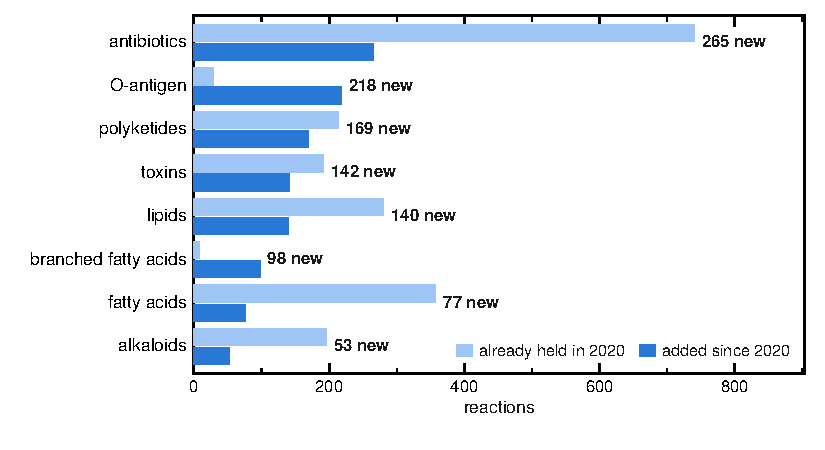
\includegraphics[width=0.85\textwidth]{../figures/figureS1_pathway_classes.pdf}
\caption{\textbf{Where the growth since 2020 landed.} Reactions from MetaCyc that were added since 2020 against those already held. Here we show the eight classes of pathways for which we added the most reactions. Growth is concentrated in specialised metabolism and cell-envelope biosynthesis.}\label{fig:s1} \end{figure}

\end{document}
